\section{Road Intersection Density}

% how density could indicate formal
% the estimated accuracy?
% add picture to explain
% how intersections found in images
% ^ theoretical background
%

As a novel approach for the distinction between formal and informal regions, we
propose the density of intersections as a metric. This is based on the belief that
areas with a dense road network, thus many intersections, are well
developed, therefore indicating a formal region. Informal regions, on the other
hand, would be characterized by a dip in the density of intersections.  

% TODO: source ???
This metric is constructed using road extraction techniques. The area of road
extraction has developed over the years, starting from 1970. A straightforward
method for road extraction is the use of edge detection. Because roads have
distinct properties due to material, design and function, the appearance of
roads are often quite in contrast to the environment. For example, on satellite
images, the homogenious black color and the regular straight lines make
roads easily identifiable from the suroundings for the human eye. Edge
detection uses the sharp contrast between a road and the roadside to identify
the road.


\subsection{Road intersection extraction methods}

Besides tradional image processing methods, another promising approach in the
detection of road networks from satellite images are Neural Networks
\cite{mangala2011extraction} \cite{mokhtarzade2007road}. A study from 2017 was
able to extract both the road network together with buildings with high
accuracy using a Convolutional Neural Network \cite{alshehhi2017simultaneous}.

We used a seperate implementation of the convolutional neural network since the
research paper did not include the software used \cite{airs}. This
implementation includes a set of images, that could be used for the training
and validation of the neural network \cite{MnihThesis}. After the training of
the network on the provided images, was used to extract the roads from our own
satellite images.  Unfortunately, the mask of the road network was erroneous as
it did not represent the road network in the provided image. The suspected
cause of this failure is the difference in the training data to our satellite
imagery data.

To illustrate the difference, the trainingset contained satellite images
obtained from partly rural area's of the state of Massachusetts in the United
States while the data used in our research is from Bangalore in India which is
mostly urban.  As a result, the geographical features and the road systems are
quite different in the two area's. This could cause the network not to
recognize the roads in the images from Bangalore. The difference in resolutions
of the two image sets could be another cause. The images of Massachusets were
of a lower resolution than the images of Bangalore which could have hindered
the neural network in the correct classification of the roads, although this is
ungrounded speculation.

\subsection{Hough Transform}
As a alterative, we used conventional image processes. The image is subjected
to a number of operations that extract the road network from the image. The
first operation is the transformation of the RGB image to grayscale values.
This is done in preparation for Otsu's method for threshold, which is able to
separate buildings from roads \cite{otsu1979threshold}. The resulting image,
displayed in Figure \ref{fig:roads_hough} is a mask of the road network in the
satellite image. From an aerial point of view, roads are straight lines of
constant width. The lines can be captured the using a Hough transform. The
Hough transform is able to detect straight lines in images and create
a mathematical definition of the lines \cite{duda1972use}.  Once the roads are
mathematically defined, determining the location of the intersection is
straightforward.

\begin{figure}
\begin{tabular}{cc}
  \subfloat{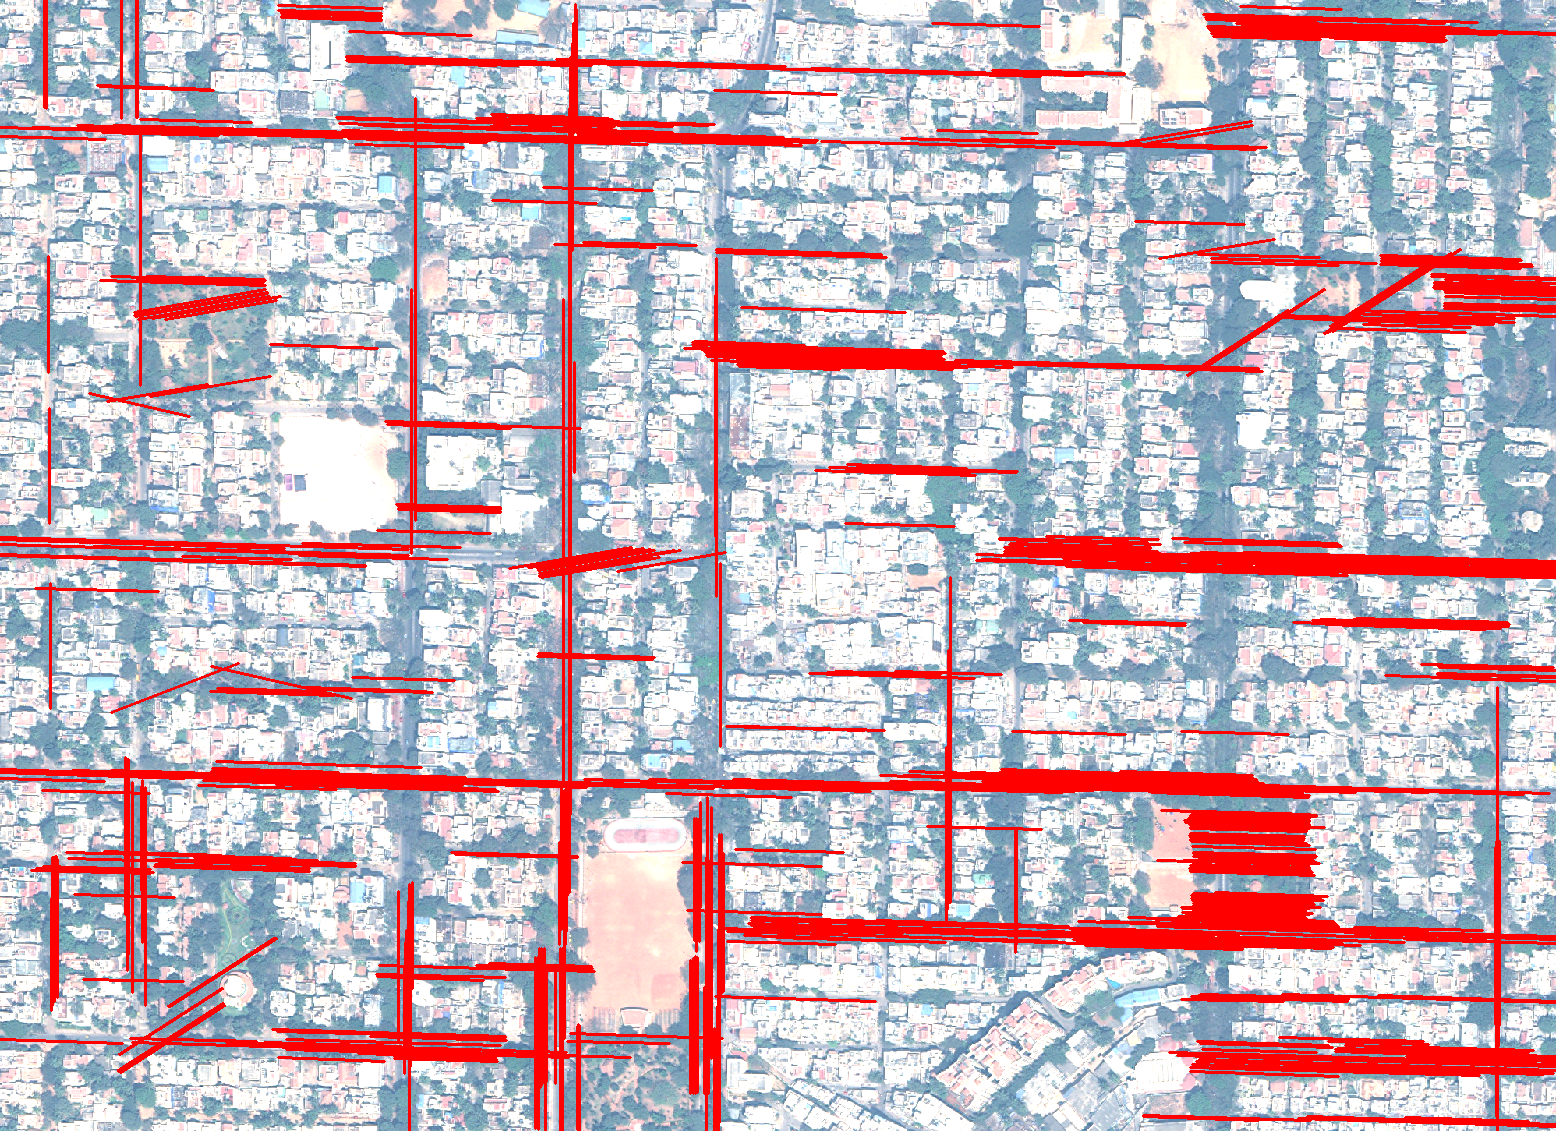
\includegraphics[width=7cm]{images/hough_road_section_8}}&
  \subfloat{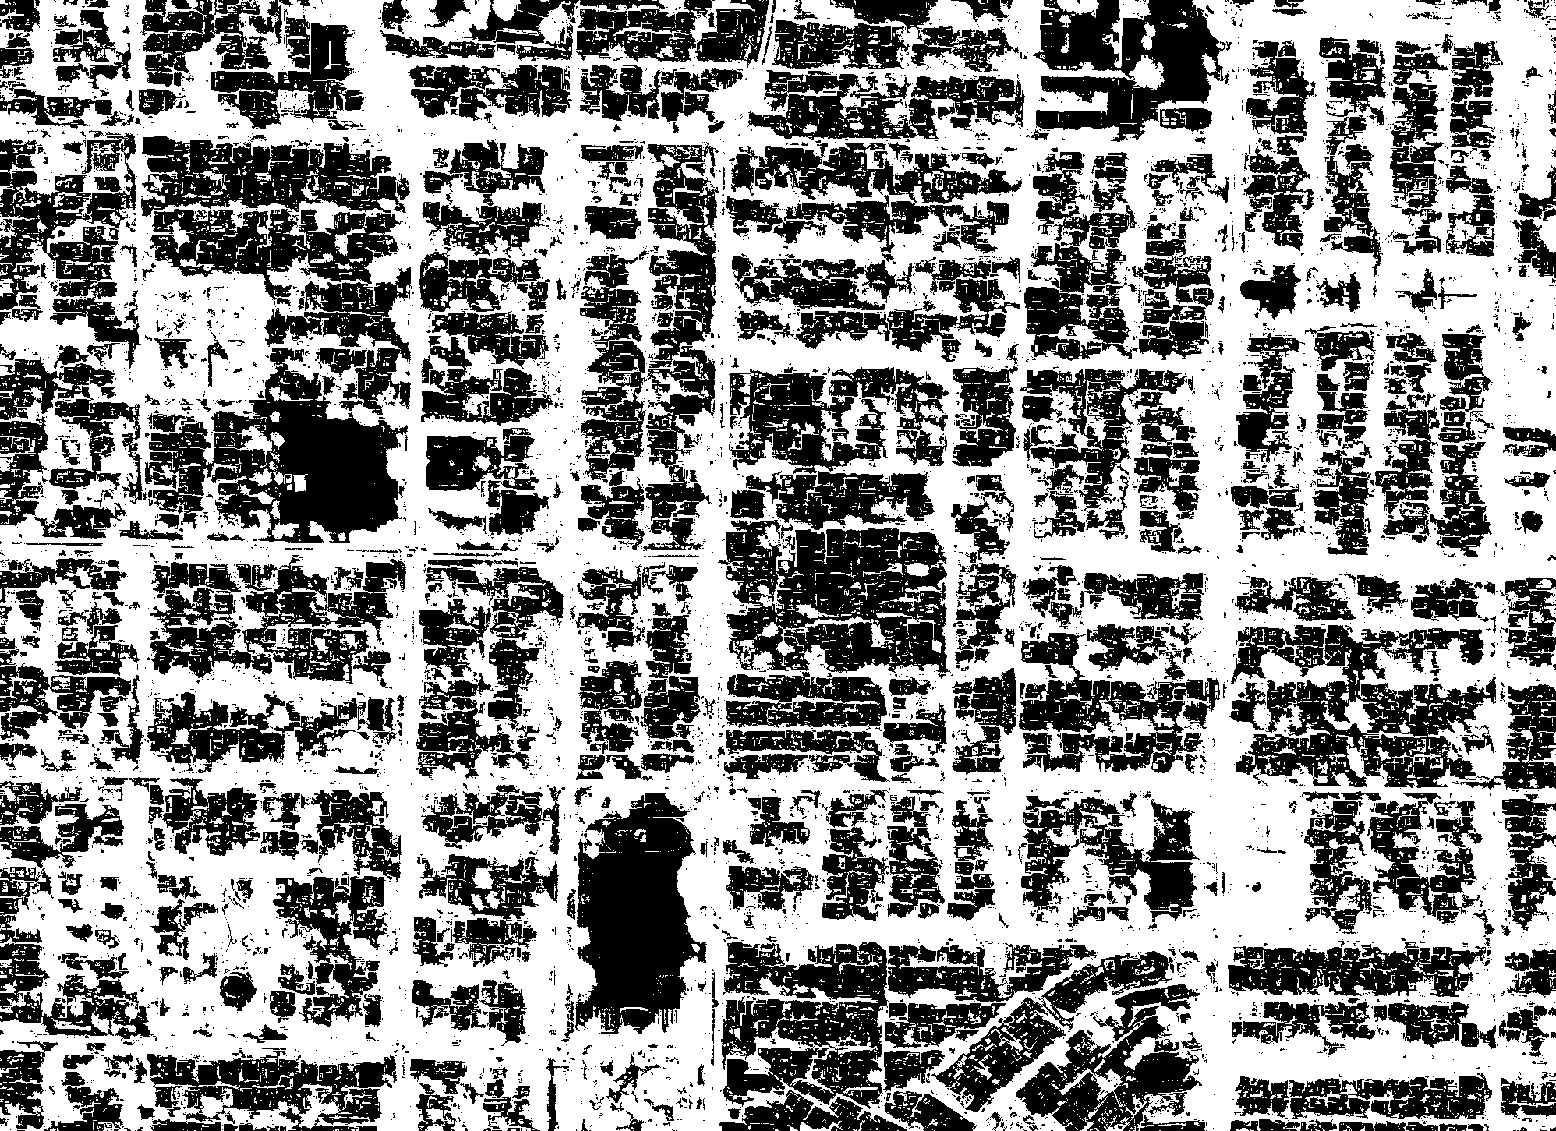
\includegraphics[width=7cm]{images/hough_road_section_8_mask}}
\end{tabular}
\caption{Detected roads using Otsu's thresholding method (left) combined with
Hough Transform (right)}
\label{fig:roads_hough}
\end{figure}

This approach was applied in practice in our research. The mask extracted
represented the road network quite accurately. The hough transform resulted in
many correct lines, although there were a lot of duplicates and noise. Although
the noise and duplicates could likely be removed for a large part, we decided
to follow a different method of intersection extraction. 

\subsection{Intersection Convolution}
We designed a new approach to detect intersections using a convolution of
a kernel with its content in the shape of an intersection. Because the kernel
matches the shape of the intersection, the output of the convolution has peaks
in the output image on the positions of the intersections. This approach has similarites to the use footprints to find the direction of
intersections \cite{hu2007road}. That paper creates certain points, called
seeds, in the image from which the road network expands using road segments.
These roadsegments can be one of a few classes, for example, a straight road,
T junction and cross intersection. The type depends on its surrounding pixels,
which form a footprint that is classified as either one of the classes. In our
research, the detection of crossroad orientation is not important, which is why
less complicated approaches can be used.

\begin{figure}%

\centering
\begin{tabular}{cc}	
	{$\displaystyle
	\begin{pmatrix}
	 0 & 0 & 0 & 1 & 1 & 0 & 0 & 0\\
	 0 & 0 & 0 & 1 & 1 & 0 & 0 & 0\\
	 0 & 0 & 0 & 1 & 1 & 0 & 0 & 0\\
	 1 & 1 & 1 & 1 & 1 & 1 & 1 & 1\\
	 1 & 1 & 1 & 1 & 1 & 1 & 1 & 1\\
	 0 & 0 & 0 & 1 & 1 & 0 & 0 & 0\\
	 0 & 0 & 0 & 1 & 1 & 0 & 0 & 0\\
	 0 & 0 & 0 & 1 & 1 & 0 & 0 & 0
	 \end{pmatrix}
	$} &
	$\vcenter{\hbox{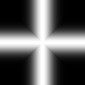
\includegraphics[width=4cm]{images/gauss_kernel}}}$
\end{tabular}

\caption{Left: Simple convolution kernel with a toe width and length of 2 and 3,
respectively. Right: Gaussian convolution kernel}%
\label{fig:conv_kernel}
\end{figure}

Before the convolution is performed, the image is first transformed to
grayscale and consequently inverted in color. In some of the  images, the grayscale version of the images already have dark roads are bright surroundings. 
However, this is not the case in every image, therefore, the otsu's thresholding is applied after the transformation to grayscale. This creates a black and white version of the image. The original kernel used for the convolution is a n by n matrix, with a cross of ones
filled with zero's, as illustrated in Figure \ref{fig:conv_kernel} on the left. To clarify
some terminology, the toe of an intersection is one of the roads leading to the
intersection. In the case of Figure \ref{fig:conv_kernel}, there are four toes
with a width and length two and three matrix cells, respectively. This kernel
has the optimal activation when it is exactly located on the same shape of the
kernel, thus cross intersections. It is therefore important to match the shape of
the kernel to the shape of the intersections in the image. This means that the
width of the toe in the kernel depends on the width of the toe of the
intersections in the image. Therefore, the dimension of the kernel depends on
the image used and the scale of the image.

\begin{figure}
\begin{tabular}{cc}
  \subfloat{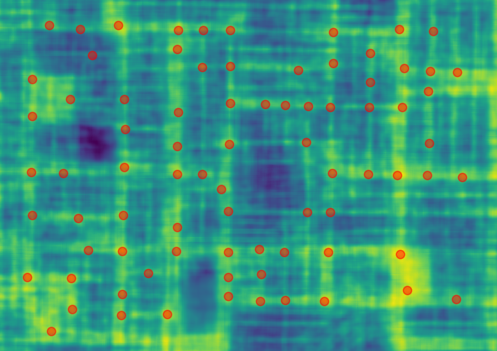
\includegraphics[width=7cm]{images/conv_road_section_8_1}}&
  \subfloat{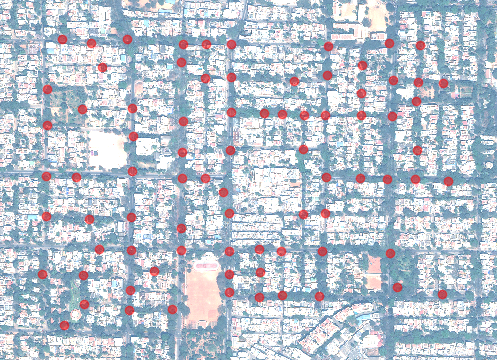
\includegraphics[width=7cm]{images/conv_road_section_8_2}}
\end{tabular}
\caption{Detection of intersections using convolution of a cross shaped kernel.
Left: Heatmap of output of the convolution; Right: Located peaks overlayed on input image}
\label{fig:roads_conv}
\end{figure}

Figure \ref{fig:roads_conv} shows the peaks of the results of the convolution
and the corresponding location of the peaks. The image used was a small section
of the image displayed in Figure \ref{fig:west-bangalore}. It was chosen
because of the regularity of the road network and with 90 degree angles between
the toes of the intersection. Furthermore, the horizontal and vertical roads
run parallel to the edges of the image. Besides, the road network is quite distinct from
the background eventhough it is quite vegetated.

The peaks in the output of the convolution are located using local maxima
detection from the python scikit-image package \cite{scikit-image}. This detects, as the name suggests, local maxima in an image. These
are regions that stand out from surrounding area. The location of these maxima
are the red dots displayed over the convolution and the corresponding input
image in Figure \ref{fig:roads_conv}.

\subsubsection{Kernels}
We have designed multiple types of kernels to extract intersection from images. In order to remove noise from the intersections, we created a new type of kernel. This kernel is similar to the kernel in figure \ref{fig:conv_kernel}, but with the zero's replaced by negative numbers. The further from the cross, the more negative the cells of the kernel become. This should therefore only capture intersections. However, when applied in practice, this kernel also seems to be activated by straight sections of road, therefore introducing a lot of noise to the intersection detection.

To account for different widths of roads in an image, we created the kernel
using gaussian distributions in contrast to the kernel displayed in Figure
\ref{fig:conv_kernel}. The kernel created using gaussian distributions is
displayed in Figure \ref{fig:gauss_kernel}.  This kernel should smooth
the contrast between roads and roadside and could remove noise. As a result of
this kernel, the center of the road is the part that counts the most. The edges
of the road are less count for less, which should help make the kernel scalable
to multiple types and sizes of roads, such as alleys or main streets.

% TODO: conclusion of kernels
%The creation of a kernel that works well for an image is 

\subsubsection{Intersection Detection Evaluation}

\begin{figure}
\begin{tabular}{cc}
  \subfloat{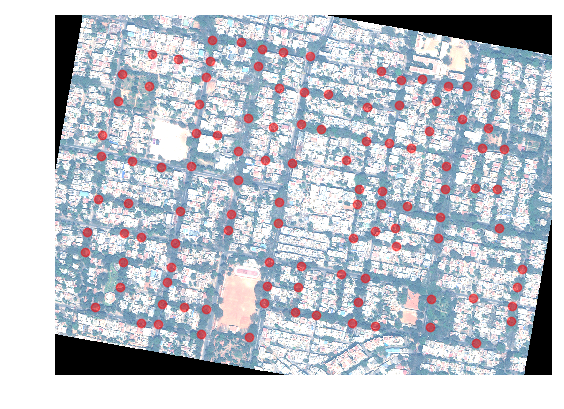
\includegraphics[width=7cm]{images/rot10}}&
  \subfloat{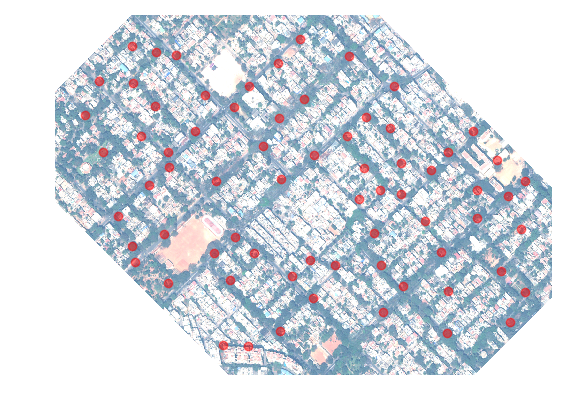
\includegraphics[width=7cm]{images/rot45}}
\end{tabular}
\caption{Performance of intersection detection in rotated intersections, from
  left to right with 10 and 45 degrees respectively}
\label{fig:roads_rot}
\end{figure}


A fundamental problem of this approach is the need to adjust the parameters to the scale and resolution of the image. Increasing the scale or resolution of an image will
change the dimensions of the intersections. Because the content of the kernel
is required to match the intersections in the image in terms of pixels, the
dimensions of the kernel should change along with change in the image. Although
the usage of the Gaussian distribution creates a more versatile kernel, it is
still required to adjust parameters according to the resolution of the image.

Because of the fixed orientation of the cross in the kernel, this approach
should inherently be prone to differences in orientation. Therefore, in the
proof of concept, we used a road system with a constant orientation, as
displayed in Figure \ref{fig:roads_conv}. Because all intersections have the
same orientation, the kernel is able to detect a large number of intersections.
However, in many other areas, the road system is not nearly as consistent.
Intersections that are rotated relative to the orientation of the kernel should
therefore be more difficult to detect. To evaluate how well this approach performs with different orientations, we
applied a rotation of 10 degrees to the image displayed in Figure
\ref{fig:roads_conv}. In the resulting image, the fast majority of
intersections were still detected, as displayed in Figure \ref{fig:roads_rot}.
The increase of the rotation to the maximum of 45 degrees results in a loss of
detections, which is as expected. Surprisingly enough, there is almost no
increase in false positives. After analysis of the output of the convolution, we believe this seemingly
invariance to rotation is caused by the method of peaks detection.  When using
the rotated image, the resulting convoluted image is more smooth with less
peaks than the unrotated image. The local maxima detection is able to
correctly detect these faint peaks in the convoluted image. Although, this approach performs reasonably well under a lot of rotation, it should primarilty be used for images with little rotation.\newline

\noindent
As mentioned earlier, the road system displayed in figures \ref{fig:roads_conv} and \ref{fig:roads_rot} do not well represent the general road network encountered in the whole of the satellite image. This becomes apparent when observing the road system in the three section displayed in Figure \ref{fig:sections}. Although the majority of land area in these sections is formal, there is a clear contrast between these road systems and the road system used in the development of this feature. The road system in the three sections are much more narrow, shorter, and less regular than the road system in \ref{fig:roads_conv}. In these sections, on many occasions, even manual extraction of intersections is quite difficult. For instance, it is often not clear whether a part of the image between two buildings is an empty strip of land or actually a road. 

Due to the different nature of the road systems, parameters used to detect the intersections in Figure \ref{fig:roads_conv} and the sections in Figure \ref{fig:sections} are different. Because the streets in these three sections are generally more narrow and less long, both the road width and road length parameters are decreased relative to the parameters used in Figure \ref{fig:roads_conv}. Furthermore, the minimum peak distance is increased to only detect peaks that are really distinct from their surroundings. The motivation behind this is to reduce noise introduced by the irregularity and obscurity of the road network.

A thorough objective evaluation of the intersection extraction could be performed due to the lack of a ground truth of the intersections. Since we are not in the posession of a groundtruth, we cannot calculate objective measures for performance, such as accuracy, recall and F1 score. Instead, the performance evaluation of the various methods and parameters used for intersection detection is based on subjective observation.

In conclusion, The use of a cross shaped kernel together with convolution seems to be able to extract the location of road intersections quite well. Although, for real world applications, such as road system mapping, this method for intersection extraction might be to simple. This method does not include the direction of the intersection. Furthermore, there is quite often noise in the extracted intersections.

% TODO: more on conclusion

% evaluation cannot metirics
% conclusion


\subsection{Feature extraction}

The estimation of the positions of intersections in an area allow for the
feature extraction of the road density. Since the objective does not concern the
precise location the intersections of a region, noise or missed intersections are not of high concern, as long as the area is well represented by the detected intersections. The density of road intersections in an area, is characterized by hotspot analysis using the Getis and Ord's local G function \cite{getis1992analysis}. The local G function is a meaure of spatial association between spatially distributed instances. In our case, these instances are the locations of the intersections. The local G function is able to detect local hotspots and coldspots in instance data, effectively indicating the location of hotspots and coldspots of the density of intersections in the image of interest.

The hotspot detection is implemented as the G function in the PySal python packackage \cite{rey2010pysal}. The feature returned from the G function is rasterized and reshaped according to the dimensions of the HoG and LSR features. Consequently, this feature can be combined with the features extracted from HoG and LSR.

% implementation in pysal?
% Leg meer uit over G functie
% leg parameters uit



